\subsection{Ejercicio 4}

  A continuaci\'on se muestran los gr\'aficos del lote 4 ejecutado en el scheduler Round-Robin.
  \begin{figure}[htb]
  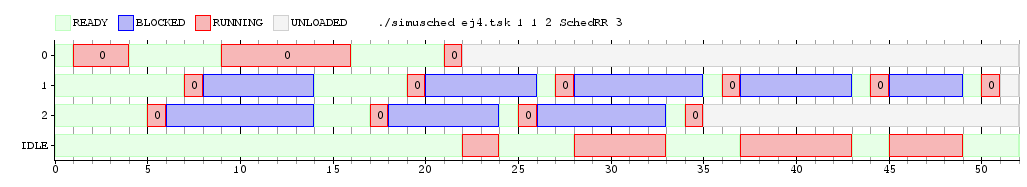
\includegraphics[scale=0.32]{images/ej4_1.png}
  \caption{Diagrama de Gantt para el lote 4 en RR con un n\'ucleo}
  \end{figure}
  \begin{figure}[htb]
  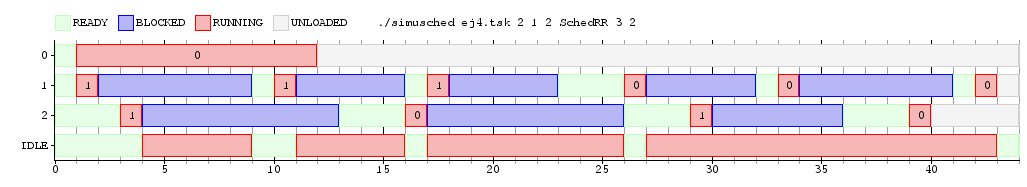
\includegraphics[scale=0.32]{images/ej4_2.png}
  \caption{Diagrama de Gantt para el lote 4 en RR con dos n\'ucleos}
  \end{figure}

  En ambos gr\'aficos se observa el comportamiento esperado de un scheduler de tipo Round-Robin. En particular, en la figura 4 se ve como la tarea 0 corre en el \'unico n\'ucleo hasta que en el tiempo 4 se le acaba
  el quantum disponible y el scheduler busca otro proceso disponible en la cola global. Tambi\'en se muestra repetidamente como cuando un proceso realiza una llamada bloqueante, el CPU deja esa tarea para ir a ejecutar
  otra. En la figura 5 se observa el mismo comportamiento, pero adem\'as podemos observar la migraci\'on de procesos entre n\'ucleos, por ejemplo a tiempo 16 en la tarea 2.
